% Created 2021-09-11 Sat 08:17
% Intended LaTeX compiler: xelatex
\documentclass[letterpaper]{article}
\usepackage{graphicx}
\usepackage{grffile}
\usepackage{longtable}
\usepackage{wrapfig}
\usepackage{rotating}
\usepackage[normalem]{ulem}
\usepackage{amsmath}
\usepackage{textcomp}
\usepackage{amssymb}
\usepackage{capt-of}
\usepackage{hyperref}
\usepackage[margin=1in]{geometry}
\usepackage{fontspec}
\usepackage{indentfirst}
\setmainfont[ItalicFont = LiberationSans-Italic, BoldFont = LiberationSans-Bold, BoldItalicFont = LiberationSans-BoldItalic]{LiberationSans}
\newfontfamily\NHLight[ItalicFont = LiberationSansNarrow-Italic, BoldFont       = LiberationSansNarrow-Bold, BoldItalicFont = LiberationSansNarrow-BoldItalic]{LiberationSansNarrow}
\newcommand\textrmlf[1]{{\NHLight#1}}
\newcommand\textitlf[1]{{\NHLight\itshape#1}}
\let\textbflf\textrm
\newcommand\textulf[1]{{\NHLight\bfseries#1}}
\newcommand\textuitlf[1]{{\NHLight\bfseries\itshape#1}}
\usepackage{fancyhdr}
\pagestyle{fancy}
\usepackage{titlesec}
\usepackage{titling}
\makeatletter
\lhead{\textbf{\@title}}
\makeatother
\rhead{\textrmlf{Compiled} \today}
\lfoot{\theauthor\ \textbullet \ \textbf{2021-2022}}
\cfoot{}
\rfoot{\textrmlf{Page} \thepage}
\titleformat{\section} {\Large} {\textrmlf{\thesection} {|}} {0.3em} {\textbf}
\titleformat{\subsection} {\large} {\textrmlf{\thesubsection} {|}} {0.2em} {\textbf}
\titleformat{\subsubsection} {\large} {\textrmlf{\thesubsubsection} {|}} {0.1em} {\textbf}
\setlength{\parskip}{0.45em}
\renewcommand\maketitle{}
\author{Albert Huang}
\date{\today}
\title{Capacitors Lab Writeup}
\hypersetup{
 pdfauthor={Albert Huang},
 pdftitle={Capacitors Lab Writeup},
 pdfkeywords={},
 pdfsubject={},
 pdfcreator={Emacs 27.2 (Org mode 9.4.4)}, 
 pdflang={English}}
\begin{document}

\maketitle
\#ret

\section{Purpose}
\label{sec:org6f0fc19}
To verify the relation between capacitance, resistance, voltage, and
charge time of a simple capacitor circuit. The equation that will be
verified is \[
V_{cap} = V_{bat}\left(1-e^{-\frac{t}{\tau}}\right)
\] where each variable has the following meaning:

\begin{center}
\begin{tabular}{lll}
Variable & Units & Description\\
\hline
\(t\) & Seconds (s) & Time elapsed since charging of the capacitor started. May be represented as \(t-t_0\), where \(t\) is the current absolute time and \(t_0\) is the absolute start time.\\
\(V_{cap}\) & Volts (V) & Voltage across the capacitor after a given elapsed time\\
\(V_{bat}\) & Volts (V) & Voltage of the battery, assumed to be constant.\\
\(\tau\) & Seconds (s) & "Time constant" that scales the equation to the circuit. Equal to the product of the resistance and capacitance of the circuit (\(RC\)), and roughly equal to the number of seconds required to charge the capacitor to \(\frac{2}{3}\) of \(V_{bat}\).\\
\end{tabular}
\end{center}

\begin{quote}
Table 1: The meanings of variables in the numerical model
\end{quote}

\section{Voltage over Time}
\label{sec:orga433a70}
\subsection{Equipment}
\label{sec:org402e18d}
\begin{itemize}
\item Logger Pro probes
\item Logger Pro
\item Breadboard
\item Capacitors (22\(\mu\)F-1000\(\mu\)F)
\item Resistors (15\(\omega\)-100k\(\omega\))
\item 3 volt battery pack
\end{itemize}

\subsection{Procedure}
\label{sec:org2318b9a}
A number of circuits were built, with the same structure but differing
resistances and capacitances. The voltage across the capacitor and the
current through the circuit were measured over time using a voltage and
amperage probe with Logger Pro.

\begin{figure}[htbp]
\centering
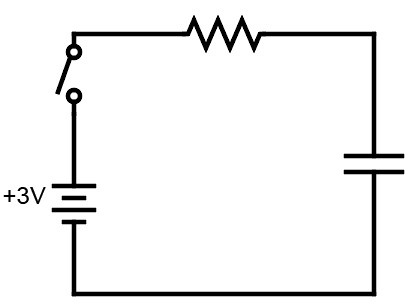
\includegraphics[width=.9\linewidth]{./KBe20phys250srcCapacitorLabCircuitSchematic.png}
\caption{Circuit Schematic}
\end{figure}

Section 3 uses a different approach to analyze this data, and Section 4
discusses the time constant as measured using a multimeter and
stopwatch, all on the same basic circuit. The raw data can be found
\href{https://nuevaschool.instructure.com/courses/2851/assignments/52558}{on
Canvas}. Desmos was used to manually fit curves to the data, using a
modified version of the model with \(t\) and \(t_0\) variables to
truncate scrap data: \[
V_{cap} = V_{bat}\left(1-e^{-\frac{t - t_0}{\tau}}\right)
\] The scattered points near the x-axis are residuals between the curve
fit and the collected data. The fit heuristic was to visually center the
dots around the x-axis.

\subsection{Results}
\label{sec:org3370aac}
The results of the fits are summarized below:

data (green). Residuals (red) were multiplied by 30.
\begin{figure}[htbp]
\centering
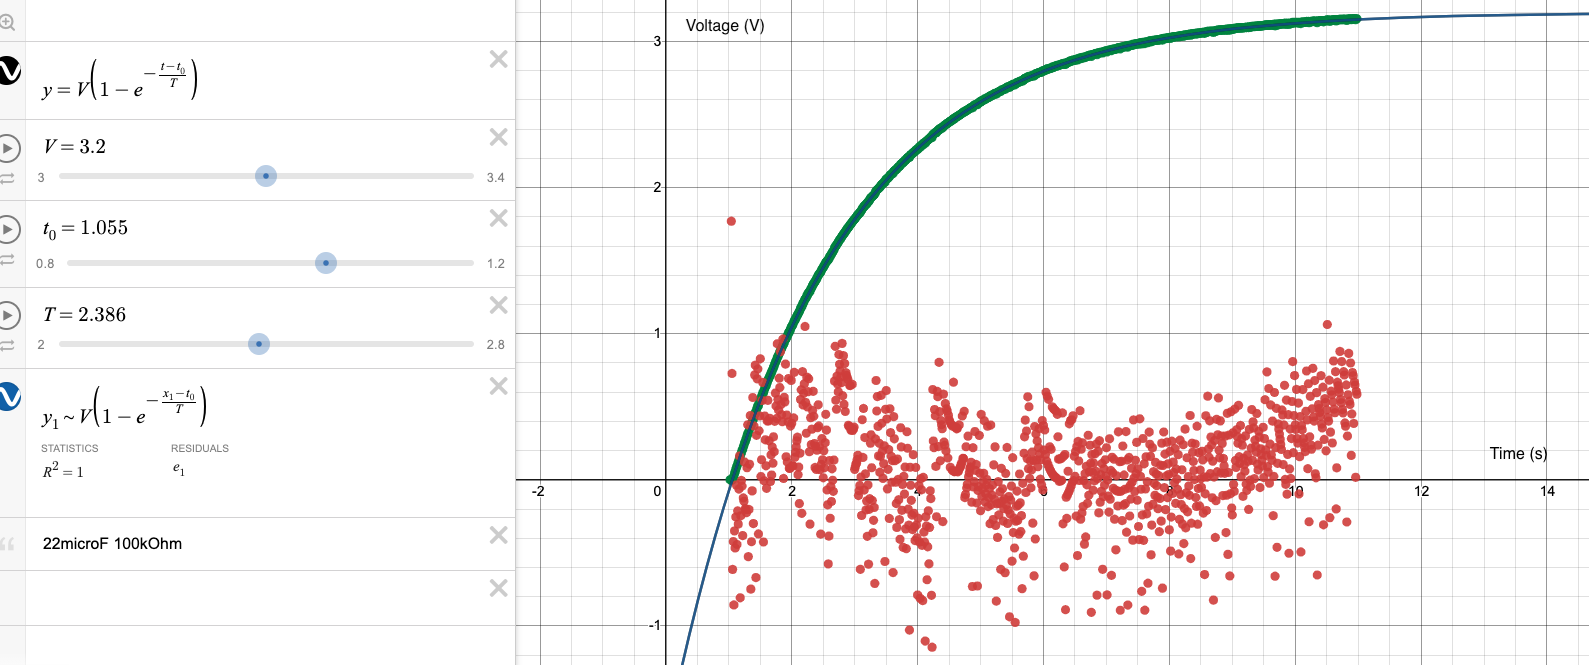
\includegraphics[width=.9\linewidth]{./KBesrcCapacitor22microF100kO.png}
\caption{Curve fit (blue) of the 100k\(\Omega\) 22\(\mu\)F circuit}
\end{figure}

(purple) of the 33\(\Omega\) 0.047\(\mu\)F data (blue). Residuals
(black) scaled x60.]]
\begin{figure}[htbp]
\centering
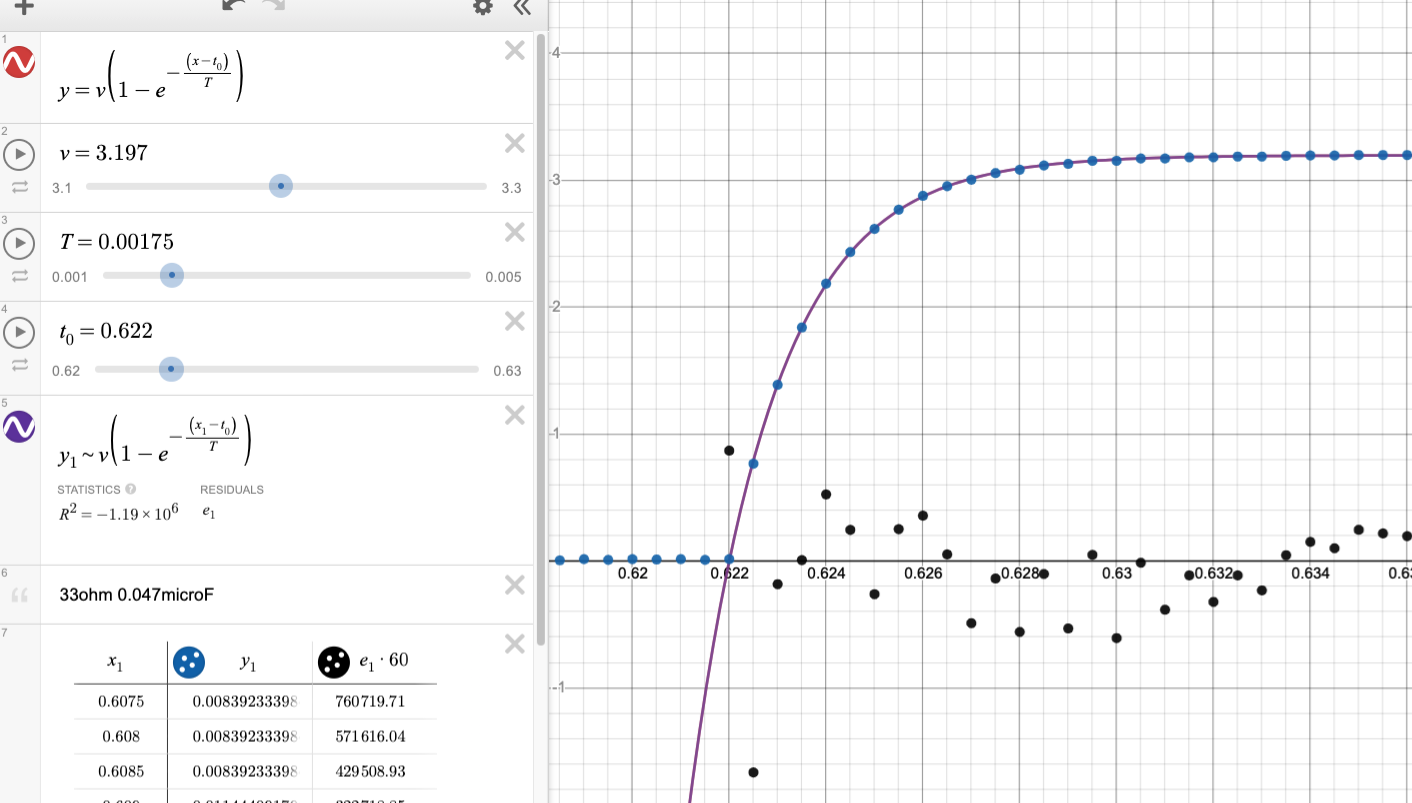
\includegraphics[width=.9\linewidth]{./KBesrcCapacitorPoint047microF33ohm.png}
\caption{[[\url{https://www.desmos.com/calculator/o3asuzdem0}][Curve fit}
\end{figure}

(black) of the 100\(\Omega\) 1000\(\mu\)F data (purple). Residuals
(blue) scaled x30.]]
\begin{figure}[htbp]
\centering
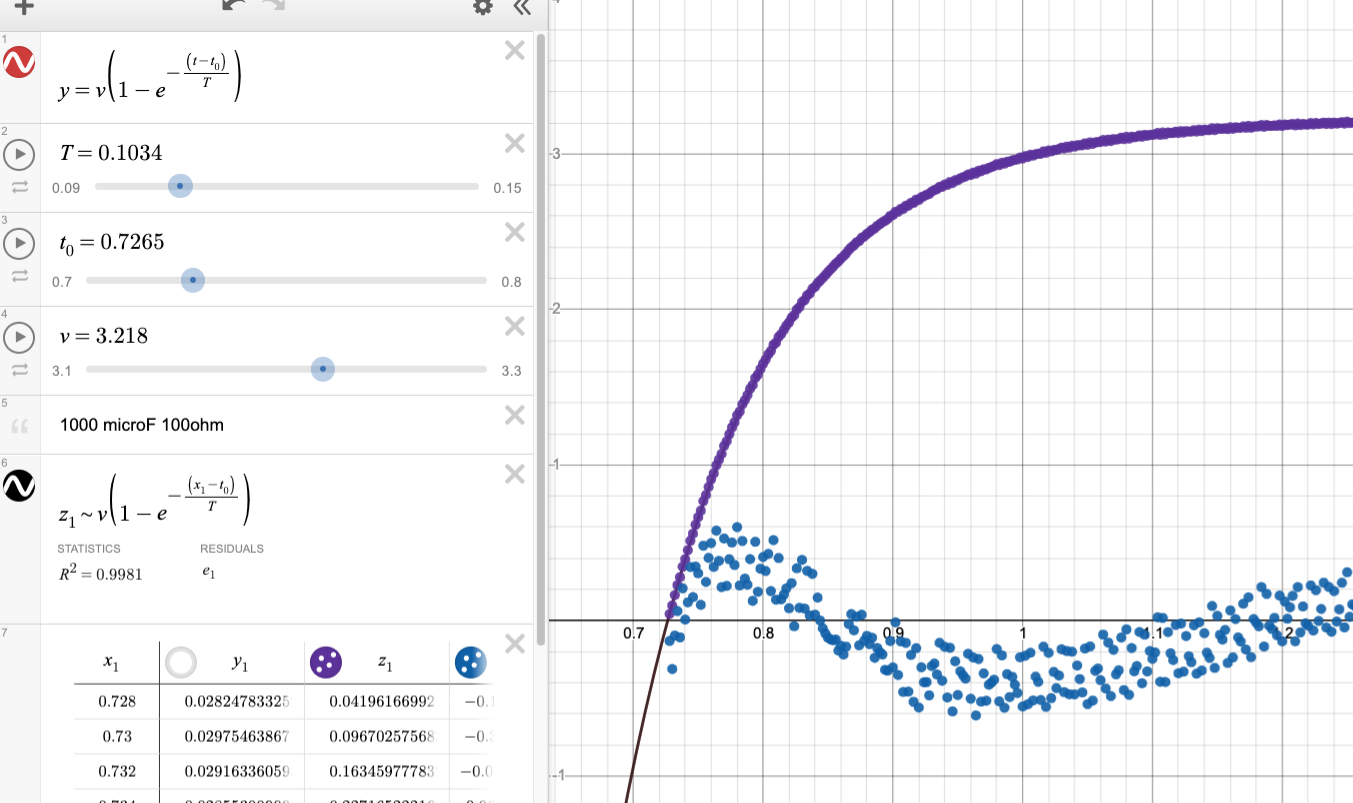
\includegraphics[width=.9\linewidth]{./KBesrcCapacitor1000microF100ohm.png}
\caption{[[\url{https://www.desmos.com/calculator/djrhxlddef}][Curve fit}
\end{figure}

(black) of the 15\(\Omega\) 1000\(\mu\)F data (purple). Residuals (red)
scaled x30.]]
\begin{figure}[htbp]
\centering
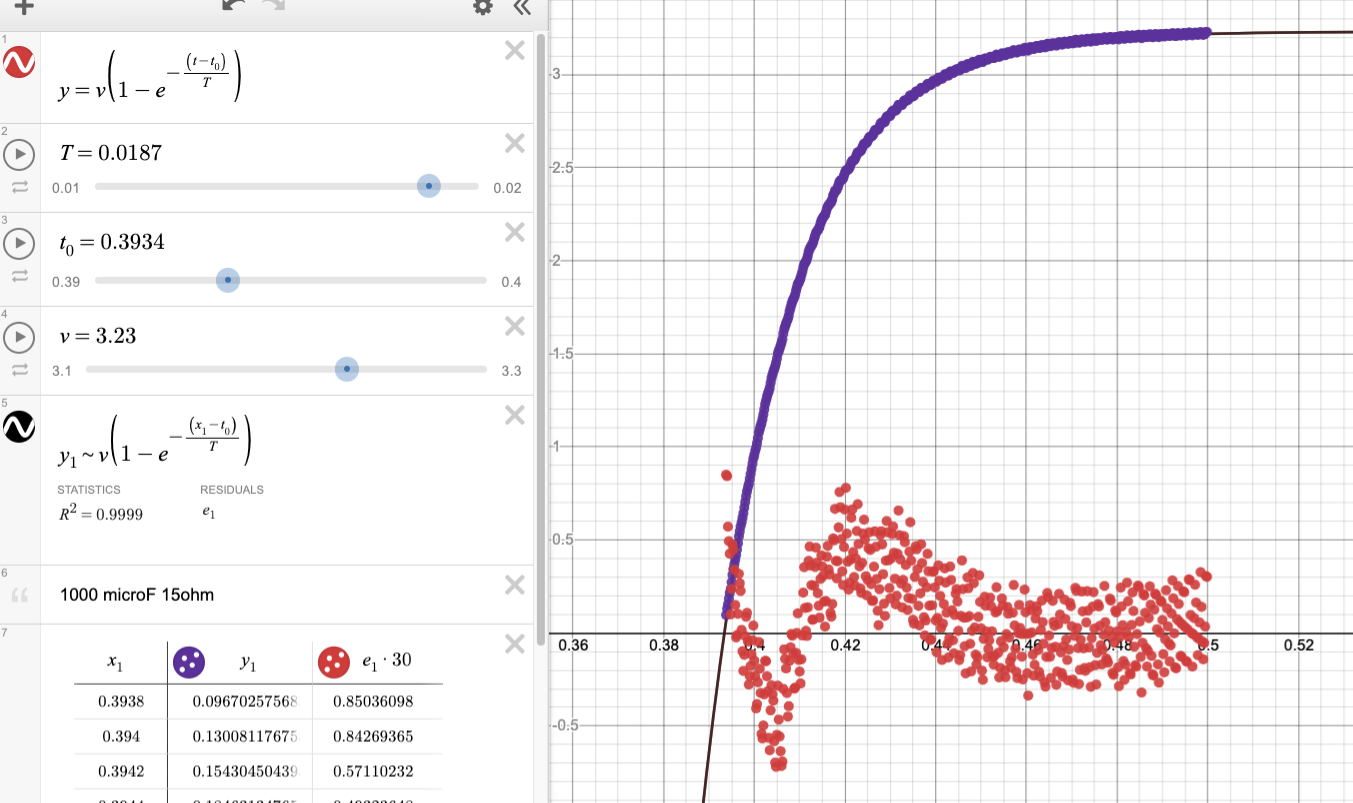
\includegraphics[width=.9\linewidth]{./KBesrcCapacitor1000microF15ohm.png}
\caption{[[\url{https://www.desmos.com/calculator/wr9bfzkbpl}][Curve fit}
\end{figure}

\begin{center}
\begin{tabular}{lllll}
\(\Omega\) & F & Fit \(\tau\) (s) & Modeled \(\tau\) (s) & \% Error\\
\hline
100k\(\Omega\) & 22\(\mu\)F & 2.3860 \(\pm\) 0.01 & 2.2000 \(\pm\) 0.441 & 8.45\%\\
33k\(\Omega\) & 0.047\(\mu\)F & 0.0017 \(\pm\) 0.0001 & 0.0016 \(\pm\) 0.0003 & 12.83\%\\
100\(\Omega\) & 1000\(\mu\)F & 0.1058 \(\pm\) 0.001 & 0.1000 \(\pm\) 0.020 & 4.40\%\\
15 \(\Omega\) & 1000\(\mu\)F & 0.0188 \(\pm\) 0.0001 & 0.0150 \(\pm\) 0.003 & 24.67\%\\
\end{tabular}
\end{center}

\begin{quote}
Table 2: Fit and calculated values of \(\tau\).
\end{quote}

\subsection{Analysis}
\label{sec:org80663ae}
The curve fits included a parameter for \(\tau\), and the model predicts
\(\tau = RC\). Thus, the values and uncertainties for resistance and
capacitance of each circuit were multiplied and compared to the visual
best fit \(\tau\) in the table above.

Because each fit was done manually, the absolute error was difficult to
estimate because there was no correct answer. Instead, error was taken
as the precision at which the number was considered "close enough" by
the human doing the curve fit. Depending on the size of the value (and
scale of the Desmos slider), this results in an absolute error ranging
from 0.1 units to 0.001 units.

These uncertainties were propagated through calculations as follows: $\backslash$[
\begin{aligned}
\delta (A+B) = \sqrt{\delta A^2 + \delta B^2}\\
\frac{\delta (AB)}{AB} = \sqrt{\left(\frac{\delta A}{A}\right)^2 + \left(\frac{\delta B}{B}\right)^2}
\end{aligned}
$\backslash$] for additive and multiplicative one operations respectively.

The manufacturing tolerances of electronic components were taken into
account as well. Resistor tolerances were based on the absolute
difference between standard resistances and those measured by a
multimeter. Capacitance tolerances were based on the tolerances of a
similar capacitor for which the
\href{http://www.paullinebarger.net/DS/Foai/Foai \%5Bradial thru-hole\%5D CD110 Series.pdf}{data
sheet} was available: the FOAI CD110 radial capacitor, which had
capacitance tolerances of \(\pm\) 20\%.

\subsection{Conclusion}
\label{sec:org9871853}
Assuming perfect capacitor manufacturing, the curve fit results fell
within uncertainties of the model predicted \(\tau\) value for all
circuits except the fit in Figure 1. This is likely due to the high
uncertainties placed on smaller scale curve fits, especially the final
trial. Furthermore, with the unexpectedly large 20\% uncertainties in
capacitance all trials fell within the uncertainties of the experiment.
Thus, the model predicted the charging behavior of capacitors over time
accurately. For future iterations, numerical errors could have been
better predicted if the specifications of the exact parts used to build
the circuit were available. Additionally, more systematic curve fit
heuristics could have been used such as RSME. The exact numerical
analysis for this section can be found
\textbf{\href{https://docs.google.com/spreadsheets/d/1Hw9ooz0CtAvTP9vtw1VT9pVyfsW39IojwwrQX94VJQY/edit?usp=sharing}{here}}.

\section{Integration of Current}
\label{sec:org45aef10}
\subsection{Procedure}
\label{sec:orgc505593}
Another way to evaluate the model is to compare the amount of
transferred charge. For this comparison, a modified equation is used:

\[
Q_{cap}=Q_{max}\left(1-e^{-\frac{t-t_{0}}{\tau}}\right)
\]

This is similar to the model used in the previous procedure, but voltage
variables are replaced with charge. Current flow through the circuit is
used as a proxy to calculate the amount of charge accumulated in the
capacitor. As before, current is measured across a resistor using a
digital probe and Logger Pro.

The amount of charge on the capacitor was calculated by taking a Riemann
sum of the momentary current measurements. In addition, the voltage
measurements across the capacitor were used as another proxy to
calculate the amount of charge on the capacitor.

\subsection{Results}
\label{sec:org5a3f94b}
The values of the three theoretically identical methods of calculating
capacitor charge are shown below:

\url{https://docs.google.com/spreadsheets/d/e/2PACX-1vRfxrZPfJZareibOZN-KammmgQDBDb5PVMBNmzCvUb\_0tSn\_TUNsLFQPM8ehfIKGEOaIhL86IoPFdb0/pubchart?oid=483417085\&format=image}

In addition, the final accumulated charge calculated by the Riemann sum
was 0.00319C, or the equivalent of 3.19V on the capacitor.

\subsection{Analysis}
\label{sec:org5519335}
As the graph shows, both proxies of charge on the capacitor generally
agree with the model but come up with smaller values of charge. Notably,
the two experimental proxies don't agree with each other either,
suggesting some systematic error is at play.

One culprit may be misaligned data: if the Riemann sum calculation began
after charging, then the entire sum would be skewed low. However, the
sum plot is not a vertical translation of the theoretical value, which
suggests the effect of this issue is minimal or canceled. Another issue
may be miscalibrated sensors: if each amperage measurement was off by
\(10^{-5}\)A, the cumulative affect would drag down the total as time
went on. The effect of this drift can be counteracted by taking the
average of readings when no charge should be flowing, multiplying by the
number of data points, and subtracting the total from the final charge
value. However, the calculated drift was an order of magnitude greater
than the total accumulated charge, so the author did not numerically
sanitize against this drift.

Although the intermediate charge values do not match the model, the
final accumulated charge is sensical: 3.19 volts is close to the
expected 3.2 volts. The same errors mentioned previously contribute to
this difference, but the accuracy of the result suggests that the effect
was canceled.

The Farad Definition line (red) in Figure 6 has blips for unkown
reasons. When the battery was off, the probe measured voltages on the
order of \(10^{-9}\) for a few ticks before measuring a faulty value, so
a similar stepping phenomenon may be occuring in the voltage
meauserement.

\subsection{Conclusion}
\label{sec:org88cf4bd}
The Riemann sums of measured current align with the model and expected
charge calculated by the voltage on the capacitor and the definition of
the Farad. Thus, the model accurately predicts experimental behavior,
suggesting that it is correct. Although the graphs differed slightly,
these may be attributed to the subjective curve fit metric, sensor
inaccuracies while measuring small flows of current, or sensor
calibration inaccuracies. Future analysis could be more accurate by
calculating the false zero point of the sensor, using various tick times
to find the most effective range for that sensor, and having more
accurate values for uncertainty for circuit components and the digital
probe.

Source analysis
\href{https://docs.google.com/spreadsheets/d/1eDmGRePGh8PVv2aKhVhv-TNJc3\_n8H7HUrAMvxOG1Vs/edit?usp=sharing}{\textbf{here}}.

\section{Time Constant with Various Components}
\label{sec:org33ef0a2}
\subsection{Equipment}
\label{sec:orgcccaa18}
\begin{itemize}
\item Breadboard
\item Capacitors (100\(\mu\)F-1000\(\mu\)F)
\item Resistors (99.8k\(\Omega\)-1M\(\Omega\))
\item 3 volt battery pack
\item Multimeter
\item Stopwatch
\end{itemize}

\subsection{Procedure}
\label{sec:orgc56f727}
Most of the analysis for data collected as a class was done on the
"charge rate constant" (\texttt{time/RC}) of each circuit, defined as:

\[
\frac{t}{RC}
\]

The same circuit as above was built by various experimentalists, with
multimeter probes on the two sides legs of the capacitor:

\begin{figure}[htbp]
\centering
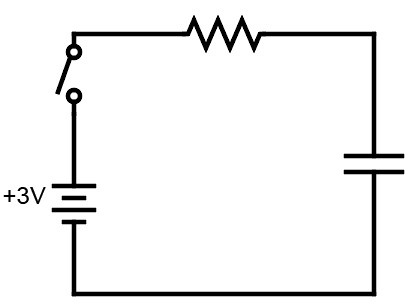
\includegraphics[width=.9\linewidth]{./KBe20phys250srcCapacitorLabCircuitSchematic.png}
\caption{Circuit Schematic}
\end{figure}

The physical manifestation of which looked like:

attached to multimeter, battery attatched to the power rails.
\begin{figure}[htbp]
\centering
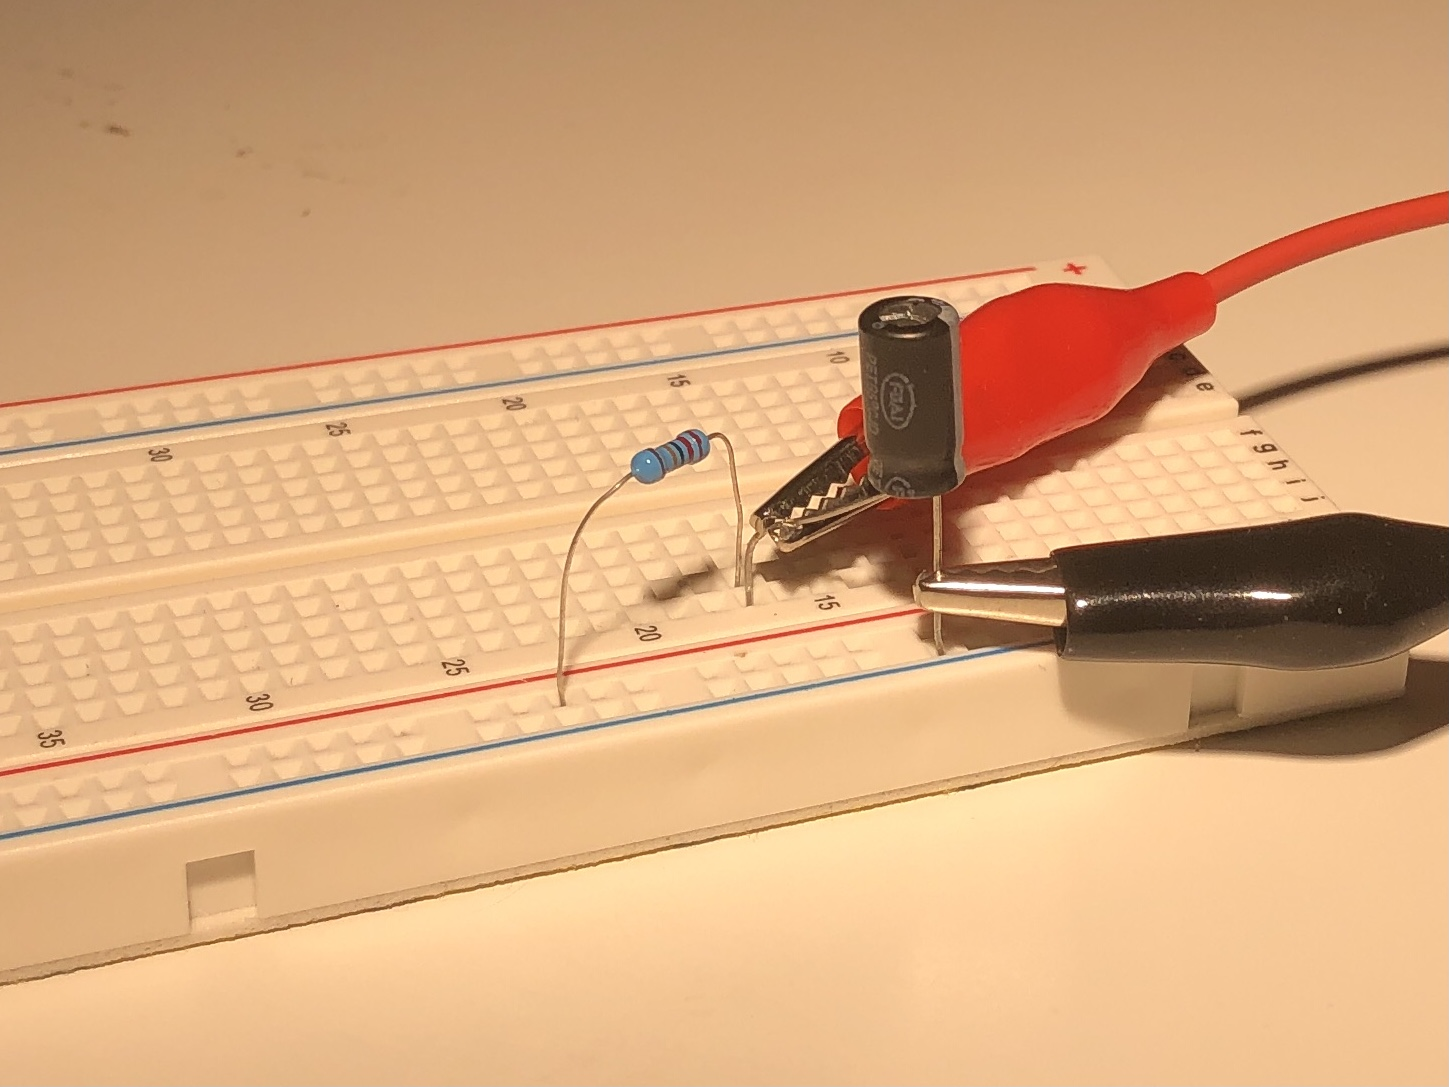
\includegraphics[width=.9\linewidth]{./KBe20phys250srcCapacitorLabCircuit.png}
\caption{Circuit used in experiment: red and black aligator clips}
\end{figure}

Starting with discharged capacitors, a battery was connected to the
circuit and used to charge the capacitor. The time taken for the voltage
across the capacitor to reach 2 \(\pm\) 0.01 volts was measured for
various resistor and capacitor combinations.

\subsection{Results}
\label{sec:org81f9fd5}
\texttt{time/RC} is a unitless scalar that represents how quickly it takes to
charge any capacitor for a given voltage. Voltage data was not collected
during the experiment, so the voltage is assumed to be constant across
trials. If our model of capacitor charge rate is correct, we expect
\texttt{time/RC} to be constant across trials. The actual data was skewed
right:

\url{https://docs.google.com/spreadsheets/d/e/2PACX-1vTdonVC\_CHgEAoezSnGLXLRFZMhR0\_IfTl8anSSMXwEDUR4iNzQbhVJGY8PyUq2e946cMuQbj5TSex\_/pubchart?oid=587065174\&format=image}

By comparing the \texttt{time/RC} and different properties of each circuit,
reasoning for the outliers may be deduced. The visualization of the
histogram is reflected in each of the following charts by the density of
points in a column.

First, the \texttt{time/RC} values were compared with the resistance of the
circuit:

\url{https://docs.google.com/spreadsheets/d/e/2PACX-1vTdonVC\_CHgEAoezSnGLXLRFZMhR0\_IfTl8anSSMXwEDUR4iNzQbhVJGY8PyUq2e946cMuQbj5TSex\_/pubchart?oid=1655543849\&format=image}

Although some outliers came from circuits with high resistance, the most
skewed ones came from those with least resistance. The same can be said
of capacitance:

\url{https://docs.google.com/spreadsheets/d/e/2PACX-1vTdonVC\_CHgEAoezSnGLXLRFZMhR0\_IfTl8anSSMXwEDUR4iNzQbhVJGY8PyUq2e946cMuQbj5TSex\_/pubchart?oid=1866933099\&format=image}

Finally, the comparison with time taken to charge the capacitor shows
the strongest correlation, which is to be expected because according to
the model, this value is the product of the previous two trends.

\url{https://docs.google.com/spreadsheets/d/e/2PACX-1vTdonVC\_CHgEAoezSnGLXLRFZMhR0\_IfTl8anSSMXwEDUR4iNzQbhVJGY8PyUq2e946cMuQbj5TSex\_/pubchart?oid=716778401\&format=image}

\subsection{Analysis}
\label{sec:org9633b2e}
On explanation for the data skew is reaction time: for lower values of
\(\tau\), the capacitor plateaus faster near 2V and thus the time keeper
may not react as quickly. Components with smaller ratings also need
tighter tolerances to achieve the same relative tolerances, so smaller
capacitors may have relatively higher manufactured variability. The
source analysis for these conclusions can be found
\href{https://docs.google.com/spreadsheets/d/1Xf3b3GKpNSIkuoEZTTcMQ2gjTIVnO4eHE5aJD3GEjqg/edit?usp=sharing}{\textbf{here}}.

\noindent\rule{\textwidth}{0.5pt}
\end{document}
